\documentclass{article}
\usepackage{graphicx} % Required for inserting images
\usepackage{fancyhdr} % Header
\usepackage{lastpage}
\usepackage[a4paper, total={6in, 8in}]{geometry}
\usepackage{float} % Floating position
\usepackage{hyperref} % Links
\usepackage{amsmath} % Math
\usepackage{amssymb} % Math
\usepackage{listings} % Import code in appendix
\usepackage{xcolor} % For coloring code
% Listing Configuration
\lstset{
    language=Python,
    basicstyle=\ttfamily\small,
    keywordstyle=\color{blue},
    stringstyle=\color{red},
    commentstyle=\color{green},
    showstringspaces=false,
    breaklines=true,
    frame=single
}
\usepackage{tikz} % Graph
\usetikzlibrary{bayesnet}
\usetikzlibrary{positioning}
\usetikzlibrary{decorations.markings}

\tikzset{
  red dot edge/.style={
    decoration={
      markings,
      mark=at position 0 with {\fill[red] circle (2pt);},
    },
    postaction={decorate},
  },
} % Red dot - place in [] just after \edge

\graphicspath{{images/}}

\newcommand{\authorFst}{Tristan Perrot}
\newcommand{\emailFst}{\href{mailto:tristanp@kth.se}{tristanp@kth.se}}
\newcommand{\authorSnd}{Étienne Riguet}
\newcommand{\emailSnd}{\href{mailto:riguet@kth.se}{riguet@kth.se}}

\pagestyle{fancy}
\fancyhf{} % clear all header and footer fields
\lhead{Assignment 1A \\ DD2434 - Machine Learning, Advanced Course}
\rhead{\authorFst \\ \authorSnd}
\cfoot{\thepage \  / \pageref{LastPage}}
\setlength{\headheight}{23pt}
\setlength{\footskip}{70pt}

\title{DD2434 - Machine Learning, Advanced Course \\ Assignment 1A}
\author{\authorFst \\ \emailFst \and \authorSnd \\ \emailSnd}
\date{November 2023}

\begin{document}

\maketitle

\begin{center}
    
\includegraphics[scale=0.5]{KTH_logo_RGB_bla.png}
\end{center}

\thispagestyle{empty}

\newpage
\tableofcontents
\newpage

\section{Exponential Family}

\subsection*{Question 1.1}

\begin{equation}
    \begin{split}
        p(x|\theta) & = h(x) \exp(\eta(\theta) \cdot T(x) - A(\eta))           \\
                    & = h(x) \exp(\eta(\lambda) \cdot T(x) - A(\eta(\lambda))) \\
                    & = h(x) \exp(\log \lambda \cdot x - A(\log \lambda))      \\
                    & = h(x) \exp(\log \lambda \cdot x - \lambda)              \\
                    & = h(x) \exp(\log \lambda \cdot x) \exp(-\lambda)         \\
                    & = e^{-\lambda} \frac{\lambda^x}{x!}
    \end{split}
\end{equation}

We can see that the distribution correspond to a \underline{Poisson distribution of parameter $\lambda$}.

\subsection*{Question 1.2}

\begin{equation}
    \begin{split}
        p(x|\theta) & = h(x) \exp(\eta(\theta) \cdot T(x) - A(\eta))                                            \\
                    & = \exp(\eta([\alpha, \beta]) \cdot [\log x, x] - A(\alpha - 1, -\beta))                   \\
                    & = \exp([\alpha - 1, -\beta] \cdot [\log x, x] - \log \Gamma(\alpha) + \alpha \log(\beta)) \\
                    & = \exp((\alpha - 1) \log x - \beta x - \log \Gamma(\alpha) + \alpha \log(\beta))          \\
                    & = \frac{\beta^\alpha}{\Gamma(\alpha)} x^{\alpha - 1} e^{-\beta x}
    \end{split}
\end{equation}

We can see that the distribution correspond to a \underline{Gamma distribution of parameters $\alpha$ and $\beta$}.

\subsection*{Question 1.3}

\begin{equation}
    \begin{split}
        p(x|\theta) & = h(x) \exp(\eta(\theta) \cdot T(x) - A(\eta))                                                                                                 \\
                    & = \frac{\exp(\eta([\mu, \sigma^2]) \cdot [x, x^2] - A(\eta([\mu, \sigma^2])))}{\sqrt{2 \pi}}                                                   \\
                    & = \frac{\exp([\frac{\mu}{\sigma^2}, - \frac{1}{2 \sigma^2}] \cdot [x, x^2] - A([\frac{\mu}{\sigma^2}, - \frac{1}{2 \sigma^2}]))}{\sqrt{2 \pi}} \\
                    & = \frac{\exp(\frac{\mu x}{\sigma^2} - \frac{x^2}{2 \sigma^2} - \frac{\mu^2}{2 \sigma^2} - \log \sigma)}{\sqrt{2 \pi}}                          \\
                    & = \frac{\exp(- \frac{(x - \mu)^2}{2 \sigma^2})}{\sigma \sqrt{2 \pi}}
    \end{split}
\end{equation}

We can see that the distribution correspond to a \underline{Normal distribution of parameters $\mu$ and $\sigma^2$}.

\subsection*{Question 1.4}

\begin{equation}
    \begin{split}
        p(x|\theta) & = h(x) \exp(\eta(\theta) \cdot T(x) - A(\eta))                        \\
                    & = 2 \exp(\eta(\lambda) \cdot x - A(\eta(\lambda)))                    \\
                    & = 2 \exp(- \lambda x - A(-\lambda))                                   \\
                    & = 2 \exp\left(- \lambda x + \log\left(\frac{\lambda}{2}\right)\right) \\
                    & = \lambda e^{- \lambda x}
    \end{split}
\end{equation}

We can see that the distribution correspond to a \underline{Exponential distribution of parameter $\lambda$}.

\subsection*{Question 1.5}

\begin{equation}
    \begin{split}
        p(x|\theta) & = h(x) \exp(\eta(\theta) \cdot T(x) - A(\eta))                                                                                     \\
                    & = \exp(\eta([\psi_1, \psi_2]) \cdot [\log x, \log (1 - x)] - A(\eta([\psi_1, \psi_2])))                                            \\
                    & = \exp([\psi_1 - 1, \psi_2 - 1] \cdot [\log x, \log (1 - x)] - A([\psi_1 - 1, \psi_2 - 1]))                                        \\
                    & = \exp((\psi_1 - 1) \log x + (\psi_2 - 1) \log (1 - x) - \log \Gamma(\psi_1) - \log \Gamma(\psi_2) + \log \Gamma(\psi_1 + \psi_2)) \\
                    & = \frac{\Gamma(\psi_1 + \psi_2)}{\Gamma(\psi_1) \Gamma(\psi_2)} x^{\psi_1 - 1} (1 - x)^{\psi_2 - 1}
    \end{split}
\end{equation}

We can see that the distribution correspond to a \underline{Beta distribution of parameters $\psi_1$ and $\psi_2$}.

\section{Dependencies in a Directed Graphical Model}

\begin{figure}[H]
    \centering
    \begin{tikzpicture}

  % Define nodes
  \node[latent] (theta) {$\theta_d$};
  \node[latent, left=of theta] (alpha) {$\alpha$};
  \node[latent, right=of theta] (z) {$Z_{d,n}$};
  \node[latent, right=of z] (w) {$W_{d,n}$};
  \node[latent, right=of w] (beta) {$\beta_k$};
  \node[latent, right=of beta] (eta) {$\eta$};

  % Connect nodes
  \edge {alpha} {theta}
  \edge {theta} {z}
  \edge {z} {w}
  \edge {beta} {w}
  \edge {eta} {beta}

  % Plates
  \plate [inner xsep=0.3cm] {plate1} {(z)(w)} {$N$}
  \plate [inner xsep=0.3cm] {plate2} {(theta)(z)(w)(plate1)} {$D$}
  \plate [inner xsep=0.2cm, xshift=0.1cm] {plate3} {(beta)} {$K$}

\end{tikzpicture}

    \caption{Graphical model of \href{https://www.jmlr.org/papers/volume3/blei03a/blei03a.pdf}{smooth LDA}.}
    \label{fig:fig1}
\end{figure}

\subsection*{Question 2.6}

The Bayes net take this form :

\begin{figure}[H]
    \centering
    \input{dgm_answers/1.2.6/1.tikz}
    \label{fig:fig2.6.1}
\end{figure}

Then, if we use the method using the d-separation, we obtain this :

\begin{figure}[H]
    \centering
    \input{dgm_answers/1.2.6/2.tikz}
    \label{fig:fig2.6.2}
\end{figure}

Therefore, we can see that $W_{d,n} \perp W_{d,n+1} | \theta_d, \beta_{1:K}$ is \underline{false}.

\begin{figure}[H]
    \centering
    \begin{tikzpicture}

  % Define nodes
  \node[latent] (theta) {$\theta_d$};
  \node[latent, left=of theta] (alpha) {$\alpha$};
  \node[latent, below=of theta] (lambda) {$\Lambda_d$};
  \node[latent, left=of lambda] (phi) {$\Phi$};
  \node[latent, right=of theta] (z) {$Z_{d,n}$};
  \node[latent, right=of z] (w) {$W_{d,n}$};
  \node[latent, right=of w] (beta) {$\beta_k$};
  \node[latent, right=of beta] (eta) {$\eta$};

  % Connect nodes
  \edge {alpha} {theta}
  \edge {theta} {z}
  \edge {z} {w}
  \edge {beta} {w}
  \edge {eta} {beta}
  \edge {phi} {lambda}
  \edge {lambda} {theta}

  % Plates
  \plate [inner xsep=0.3cm] {plate1} {(z)(w)} {$N$}
  \plate [inner xsep=0.3cm] {plate2} {(theta)(lambda)(z)(w)(plate1)} {$D$}
  \plate [inner xsep=0.2cm, xshift=0.1cm] {plate3} {(beta)} {$K$}

\end{tikzpicture}

    \caption{Graphical model of \href{https://aclanthology.org/D09-1026.pdf}{Labeled LDA}.}
    \label{fig:fig2}
\end{figure}

\section{CAVI}

\begin{figure}[H]
    \centering
    \begin{tikzpicture}

  % Define nodes
  \node[latent] (x) {$x$};
  \node[latent, above=of x] (mu) {$\mu$};
  \node[latent, right=of mu] (tau) {$\tau$};
  \node[above=of mu] (mu_0) {$\mu_0$};
  \node[left=of mu_0] (lambda_0) {$\lambda_0$};
  \node[above=of tau] (a_0) {$a_0$};
  \node[right=of a_0] (b_0) {$b_0$};

  % Connect nodes
  \edge {mu} {x}
  \edge {tau} {x}
  \edge {a_0} {tau}
  \edge {b_0} {tau}
  \edge {lambda_0} {mu}
  \edge {mu_0} {mu}

  % Plates
  \plate [inner xsep=0.3cm, inner ysep=0.3cm] {plate1} {(x)} {$N$}

\end{tikzpicture}

    \caption{DGM}
    \label{fig:fig3}
\end{figure}

\subsection*{Question 3.12}

In the bishop book, we can see that :

\begin{equation}
    p(X|\mu, \tau) = \left(\frac{\tau}{2\pi}\right)^{N/2} \exp\left\{-\frac{\tau}{2}\sum_{n=1}^{N}(x_n - \mu)^2\right\}
\end{equation}

\begin{equation}
    p(\mu|\tau) = \mathcal{N}(\mu|\mu_0, (\lambda_0 \tau)^{-1})
\end{equation}

\begin{equation}
    p(\tau) = \text{Gam}(\tau|a_0, b_0)
\end{equation}

Then, by using the code in appendix \ref{alg:cavi}, we obtain :

\begin{figure}[H]
    \centering
    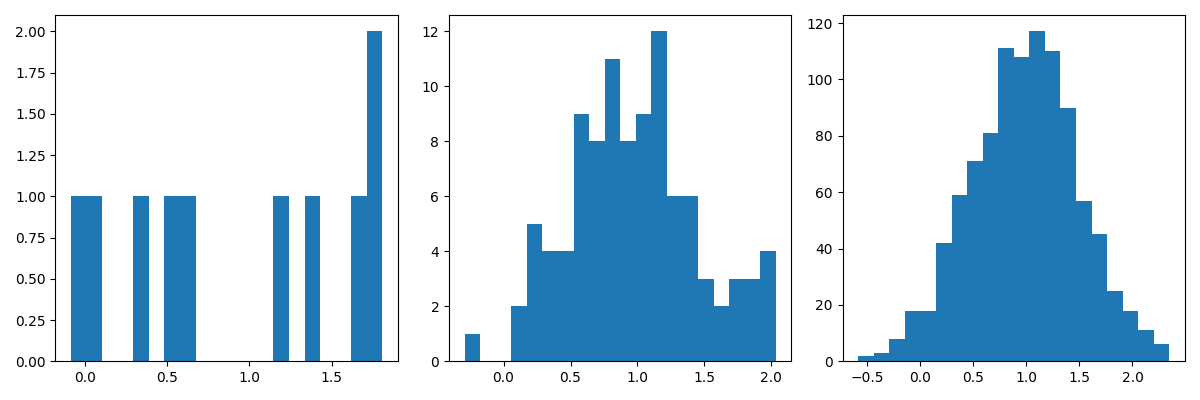
\includegraphics[scale=0.5]{py_files/12_data.png}
    \caption{Generated Data.}
    \label{fig:3.12}
\end{figure}

\subsection*{Question 3.13}

Let's find the ML estimates of $\mu$ and $\tau$.
We know that $\log(q^*(\mu)) = \mathbb{E}[\log p(X, \mu, \tau)]$.
Then, we can write :

\begin{equation}
    \begin{split}
        \log(q^*(\mu)) & = \mathbb{E}[\log p(X, \mu, \tau)]                                                                                          \\
                       & \overset{+}{=} \mathbb{E}[\log p(X|\mu, \tau)] + \mathbb{E}[\log p(\mu|\tau)]                                               \\
                       & = \mathbb{E}\left[\left(\frac{\tau}{2\pi}\right)^{N/2} \exp\left\{-\frac{\tau}{2}\sum_{n=1}^{N}(x_n - \mu)^2\right\}\right] \\
    \end{split}
\end{equation}

\newpage
\appendix

\section*{Appendix}
\addcontentsline{toc}{section}{Appendix}
\subsection*{Python Code}\label{appendix:code}
\lstinputlisting[label = {alg:cavi}]{py_files/cavi.py}

\end{document}